Writing both euations in matrix form
\begin{align}
    \myvec{4 & -3}\vec{x}=3\\
    \myvec{3 & -5}\vec{x}=7
\end{align}
Forming the augmented matrix and reducing the matrix to row echelon form:
\begin{align}
\myvec{4 & -3 & 3\\3 & -5 & 7}\\
\xleftrightarrow[]{R_1\leftarrow R_1/4}
\myvec{1 & -3/4 & 3/4\\3 & -5 & 7}\\
\xleftrightarrow[]{R_2\leftarrow R_2-3R_1}   
\myvec{1 & -3/4 & 3/4\\0 & -11/4 &19/4}\\
\xleftrightarrow[]{R_2\leftarrow R_2\times-4/11}
\myvec{1 & -3/4 & 3/4\\0 & 1 &-19/11}\\
\xleftrightarrow[]{R_1\leftarrow R_1+3/4\times R_2}
\myvec{1 & 0 & -6/11\\0 & 1 &-19/11} \label{eq:solutions/det/60/7}
\end{align}
Here, $Rank(A)=Rank(A|B)$. Therefore, the system is consistent. Also, there exist a unique solution as $Rank(A)=n$ (number of unknown).\\ 
From equation \ref{eq:solutions/det/60/7}, we get:
\begin{align}
    \vec{x}=\frac{1}{11}\myvec{-6\\-19}
\end{align}
Plotting the lines and the intersection point in Fig. \ref{Fig4:solutions/det/60/}

\begin{figure}[h!]
\centering
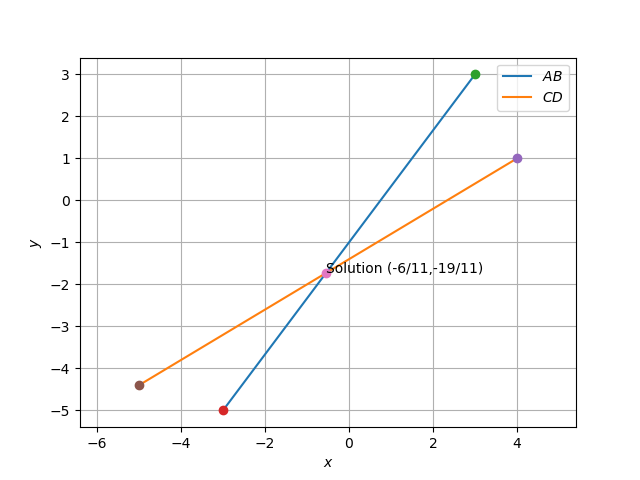
\includegraphics[width=\columnwidth]{./solutions/det/60/Figure_31}
\caption{Lines and their intersection denoting the solution}
\label{Fig4:solutions/det/60/}
\end{figure}
